\chapter{Procedures} 
\label{procedures}  
\section{Evacuating Transfer lines}
Helium transfer lines (TLs) are vacuum insulated tubes.  One end is plunged directly into a helium dewar while the other delivers liquid helium to a vessel, with a pressure differential driving the helium through.  If the vacuum jacket is compromised, the helium will cool the outer shell of the TL and frost up (helium will of course stop transferring).  Once this happens, the only solution is to remove and warm up the transfer line and evacuate the vacuum space.


TLs are evacuated with a leak checker until the leak rate plateaus.  It is recommended to pump overnight, but in a bind it can be done quicker.  An evacuated TL will be fine for months, but in practice it is safer to pump down each TL a few days before beginning a cooldown in case the vacuum space was somehow compromised in storage/transport.


\subsection{Cryofab TLs}

Cryofab TLs have a proprietary vacuum pumpout ports which require a special adapter to KF (Figure \ref{fig:cf-adapter}).

\begin{figure}[h]
 \centering
 \begin{minipage}{.45\textwidth}
 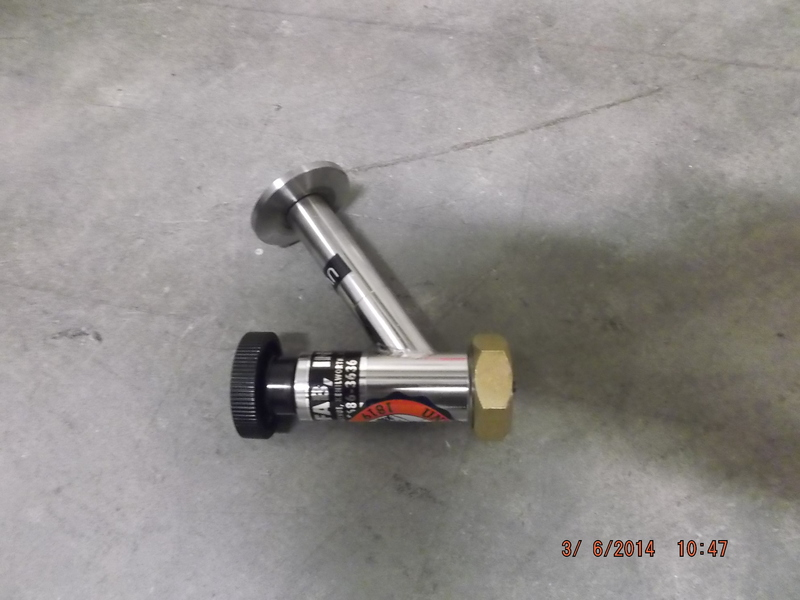
\includegraphics[width=\textwidth]{./img/cf-adapter.JPG}
 % cf-adapter.JPG: 800x600 pixel, 72dpi, 28.22x21.17 cm, bb=0 0 800 600
 \end{minipage}
 \quad
  \begin{minipage}{.45\textwidth}
 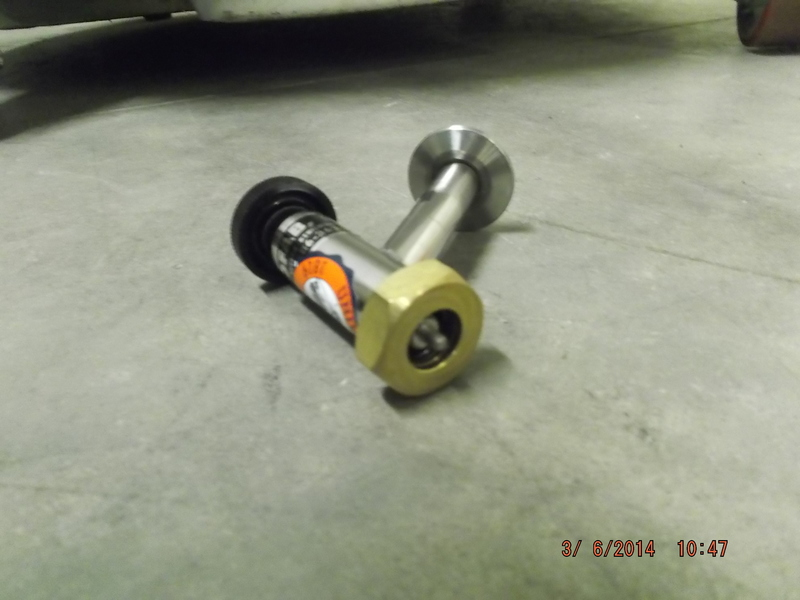
\includegraphics[width=\textwidth]{./img/cf-adapter-angle.JPG}
 % cf-adapter.JPG: 800x600 pixel, 72dpi, 28.22x21.17 cm, bb=0 0 800 600
 \end{minipage}
 \caption{The Cryofab transfer line vacuum space to KF-25 adapter with stem pushed all the way in.  The brass nut fits a 1-\nicefrac{3}{16}\inches{} wrench.}
 \label{fig:cf-adapter}

\end{figure}

To pump out the vacuum space:

\begin{enumerate}
 \item Warm up the LD.
 \item Set the TL on the ground.
 \item Loosen the brass fitting on the adapter (do not loosen all the way or the o-ring will fall out).
 \item Pull the adapter stem out about an inch and fit the adapter on the TL pumpout until almost the entire vacuum jacket pumpout is covered (Figure \ref{fig:cf-adapter-on-tl}).
 \item Tighten the brass nut.
 \item Support the weight of both ends of the TL on stable objects and attach the KF adapter to the leak checker (we use a chair and lab bench in Figure \ref{fig:cf-adapter-pushedin}).  Do not allow the TL to torque about the adapter or the TL and adapter may both be damaged.
 \item Push the stem in.
 \item Screw in the stem about 5 turns (count them if this is your first time) while gently pushing in so the threads grab.  The threads are tightening when the stem is pulled in slightly each turn.
 \item Gently pull the stem out half an inch.  \textbf{If you pull too far you will break the adapter; see Figure \ref{fig:cf-adapter-pulledout}.} If TL was under vacuum, you will hear a hiss indicating the vacuum jacket is vented.  
 \item Start the LD pump and wait for 2 minutes.  This should bring the LR to a low enough value to detect an external leak.  Spray both vacuum connections on the adapter with helium.
 \item If the KF joint leaks, clean it and try again.  If the TL-to-adapter joint leaks, either a) the adapter is not entirely over the TL pump out port or b) the brass nut is not tight enough.  Try again.
 \item Pump until the LR stops declining, preferably overnight.
 \item Again, spray both joints with helium gas.  Start over and remake the offending connection if necessary.
 \item Flow helium gas through the TL (if there is a valve like Figure \ref{fig:cf-tl-pumpout}, open it first).  If there is a leak between the inner cavity of the TL and the vacuum space the TL is broken and not suitable for a cooldown.
\end{enumerate}

Athe end of leak checking, use the following procedure to disconnect the TL from the LD:

\begin{enumerate}
 \item Push the stem straight in all way.
 \item Vent the LD.  If there is a long hiss, the stem was not pushed in all the way and the vacuum space is now filled with air.  A short hiss indicates only the small volume in the KF adapter was vented (this is good).
 \item Unscrew the stem.  If you counted the number of turns in the above section, you know how many times to unscrew it.  Otherwise, just turn a few dozen times to be sure.  Not entirely unscrewing the stem will result in the TL being entirely vented in the next step.
 \item Pull the stem back about an inch.  \textbf{If you pull too far you will break the adapter; see Figure \ref{fig:cf-adapter-pulledout}.}  You should not hear a hiss.
 \item Disconnect the KF connection from the LD and set the TL on the ground.  This may require two people to do safely depending on the weight of the TL.  Be careful not to bump the TL.
 \item Loosen the brass nut about two turns and wiggle the adapter off the TL.  Unscrewing the nut too much will make the connector fall apart; \textbf{unscrewing too little will break the adapter and/or TL if you try forcing it off}.  Do not try forcing it.
\end{enumerate}


\begin{figure}[h]
 \centering
  \begin{minipage}{.45\textwidth}
 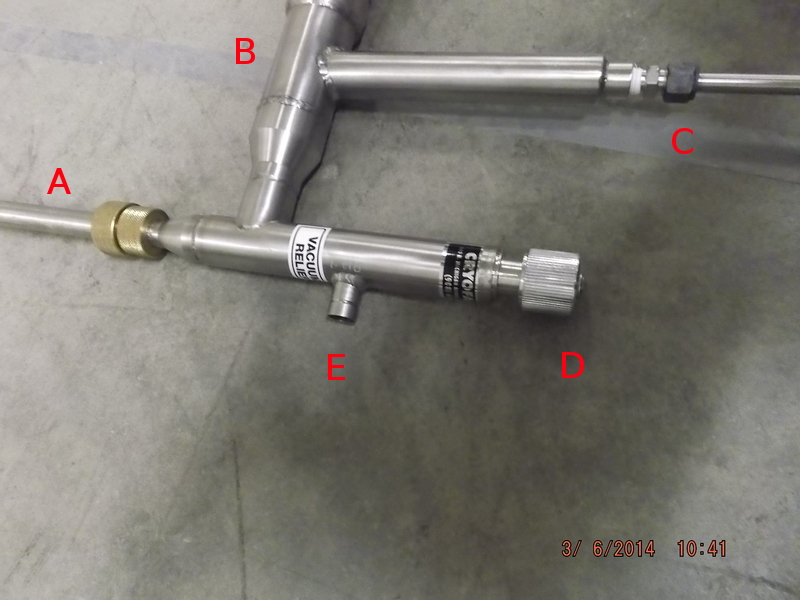
\includegraphics[width=\textwidth]{./img/cf-tl-pumpout.JPG}
 % cf-adapter-on-tl.JPG: 800x600 pixel, 72dpi, 28.22x21.17 cm, bb=0 0 800 600
 \caption{A: to TL stinger; B: to TL bayonet; C: emergency popoff valve; D: LHe flow valve; E: vacuum jacket pumpout.}
 \label{fig:cf-tl-pumpout}
 \end{minipage}
 \quad
 \begin{minipage}{.45\textwidth}
 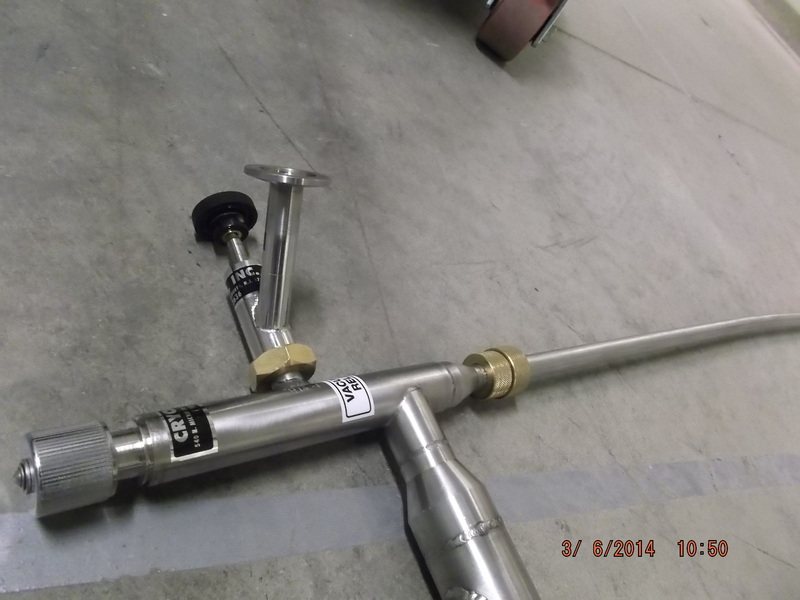
\includegraphics[width=\textwidth]{./img/cf-adapter-on-tl.JPG}
 % cf-adapter-on-tl.JPG: 800x600 pixel, 72dpi, 28.22x21.17 cm, bb=0 0 800 600
 \caption{Adapter on vacuum jacket pumpout.}
 \label{fig:cf-adapter-on-tl}
 \end{minipage}
 \quad
 \begin{minipage}{.45\textwidth}
 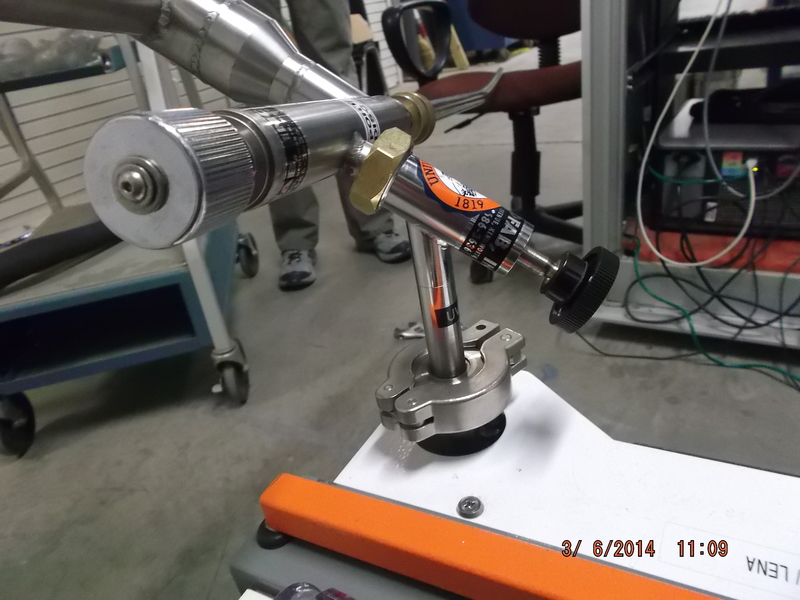
\includegraphics[width=\textwidth]{./img/cf-adapter-pushedin.JPG}
 % cf-adapter-on-tl.JPG: 800x600 pixel, 72dpi, 28.22x21.17 cm, bb=0 0 800 600
 \caption{Stem pushed in.}
 \label{fig:cf-adapter-pushedin}
 \end{minipage}
 \quad
 \begin{minipage}{.45\textwidth}
  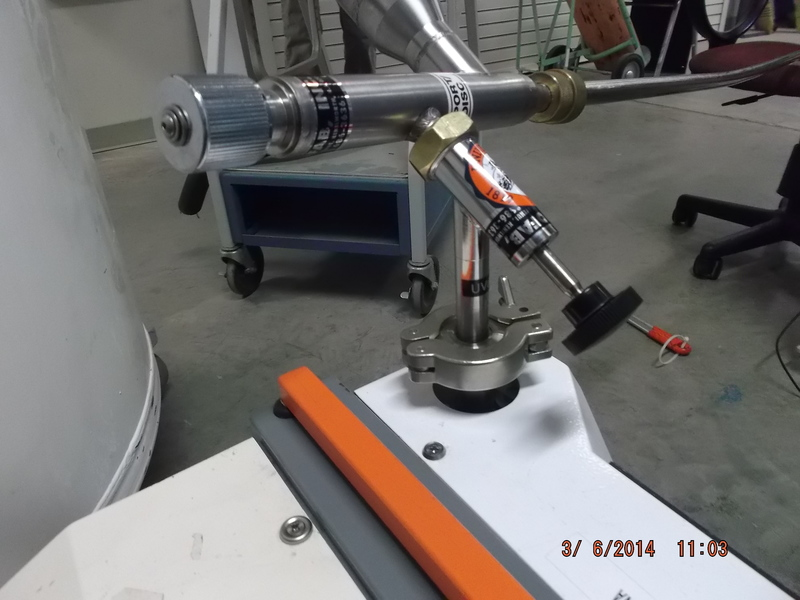
\includegraphics[width=\textwidth]{./img/cf-adapter-pulledout.JPG}
 % cf-adapter-on-tl.JPG: 800x600 pixel, 72dpi, 28.22x21.17 cm, bb=0 0 800 600
 \caption{Stem pulled out.}
 \label{fig:cf-adapter-pulledout}
 \end{minipage}
 \quad
 \end{figure}


\subsection{LTL}

The LTL, named for its shape (Figure \ref{fig:ltl}), was designed at CERN.  It did not come with a vacuum pump out adapter, so we made one by modeling the brass screw that plugs the pump port.

\begin{figure}
\begin{minipage}{.45\linewidth}
 \centering
 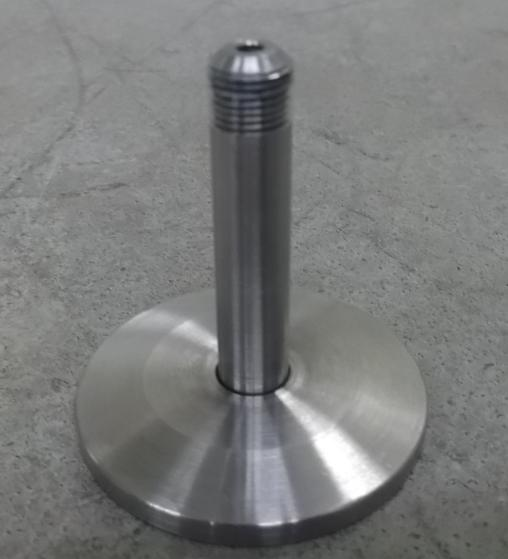
\includegraphics[width=\linewidth]{img/ltl-adapter.jpg}
 % ltl-adapter.jpg: 508x559 pixel, 762dpi, 1.69x1.86 cm, bb=0 0 48 53
 \caption{The LTL adapter.}
 \label{fig:ltl-adapter}
\end{minipage}
\quad
\begin{minipage}{.45\linewidth}
 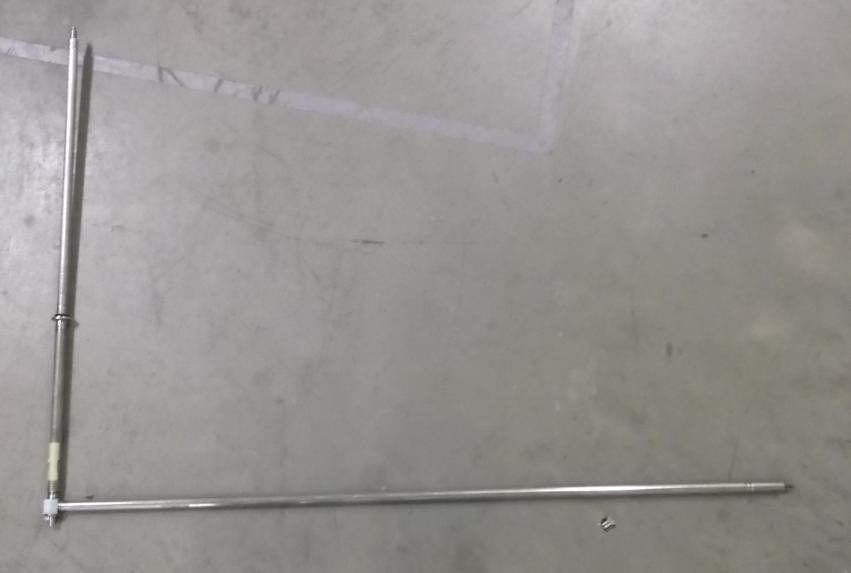
\includegraphics[width=\linewidth]{img/ltl.jpg}
 % ltl.jpg: 851x573 pixel, 762dpi, 2.84x1.91 cm, bb=0 0 80 54
 \caption{The LTL.}
 \label{fig:ltl}
\end{minipage}
\end{figure}

\begin{minipage}{\linewidth}
Gather the following:

\begin{itemize}
 \item LTL
\item KF adapter to LTL
\item teflon tape
\item flathead screwdriver
\item leak detector (LD) with KF25 oring/clamp
\item ziplock bag
\end{itemize}
\end{minipage}


\begin{enumerate}
 \item Warm up the LD.
\item Wrap the KF adapter's threads with one or two layers of teflon tape.  Do not block the tapered end with tape or it might ruin the seal.
\item Remove the top screw from the LTL and place it in the ziplock bag.
\item Open side screw valve 3 turns to break the vacuum.  If there is a hiss, the LTL was holding a vacuum.
\item Hand tighten the adapter in the top hole while being careful not to let the emergency popoff valve fall out.  It might be tricky to get the threads right with the tape between them, but do not strip the threads!
\item Start pumping with the LD.  The leak rate should should very quickly approach 10E-8.
\item After a few minutes of pumping, spray the KF and threaded joints with He gas to make sure the connection is leak tight.  If the threaded joint is leaking, \textbf{carefully} rotate the LTL \nicefrac{1}{8} of a turn, up to \nicefrac{1}{4} turn max.  If the joint is still leaking, the teflon tape will have to be removed and reapplied.
\item Pump overnight.
\item Close side screw valve and tighten.
\item Stop and vent LD and break the KF connection.
\item Unscrew the LTL adapter, making sure there is no teflon left over in the LTL port, and screw the brass top screw back in place.
\item Remove all teflon tape from the adapter.
\end{enumerate}


\begin{figure}
 \centering
 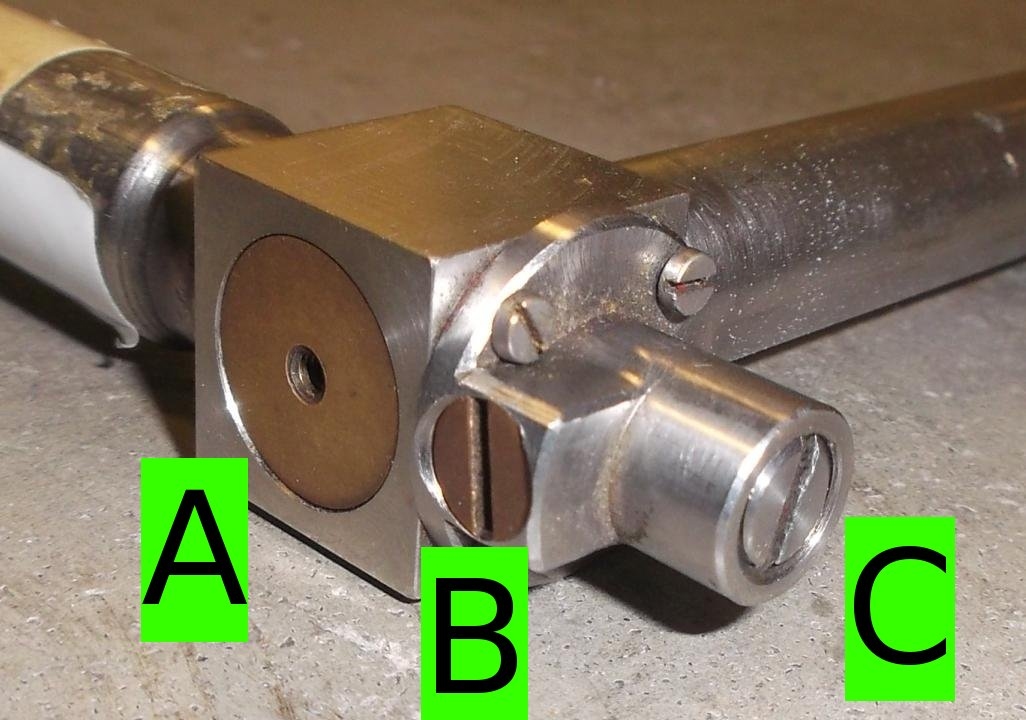
\includegraphics[width=.80\linewidth]{img/ltl-ports.jpg}
 % ltl-ports.jpg: 1026x720 pixel, 72dpi, 36.19x25.40 cm, bb=0 0 1026 720
 \caption{The three ports on the LTL: A) emergency relief popoff (this will shoot very high when the LTL freezes!), B) vacuum jacket pump port and brass placeholder screw, C) side screw valve.}
 \label{fig:ltl-ports}
\end{figure}

\begin{figure}
 \centering
 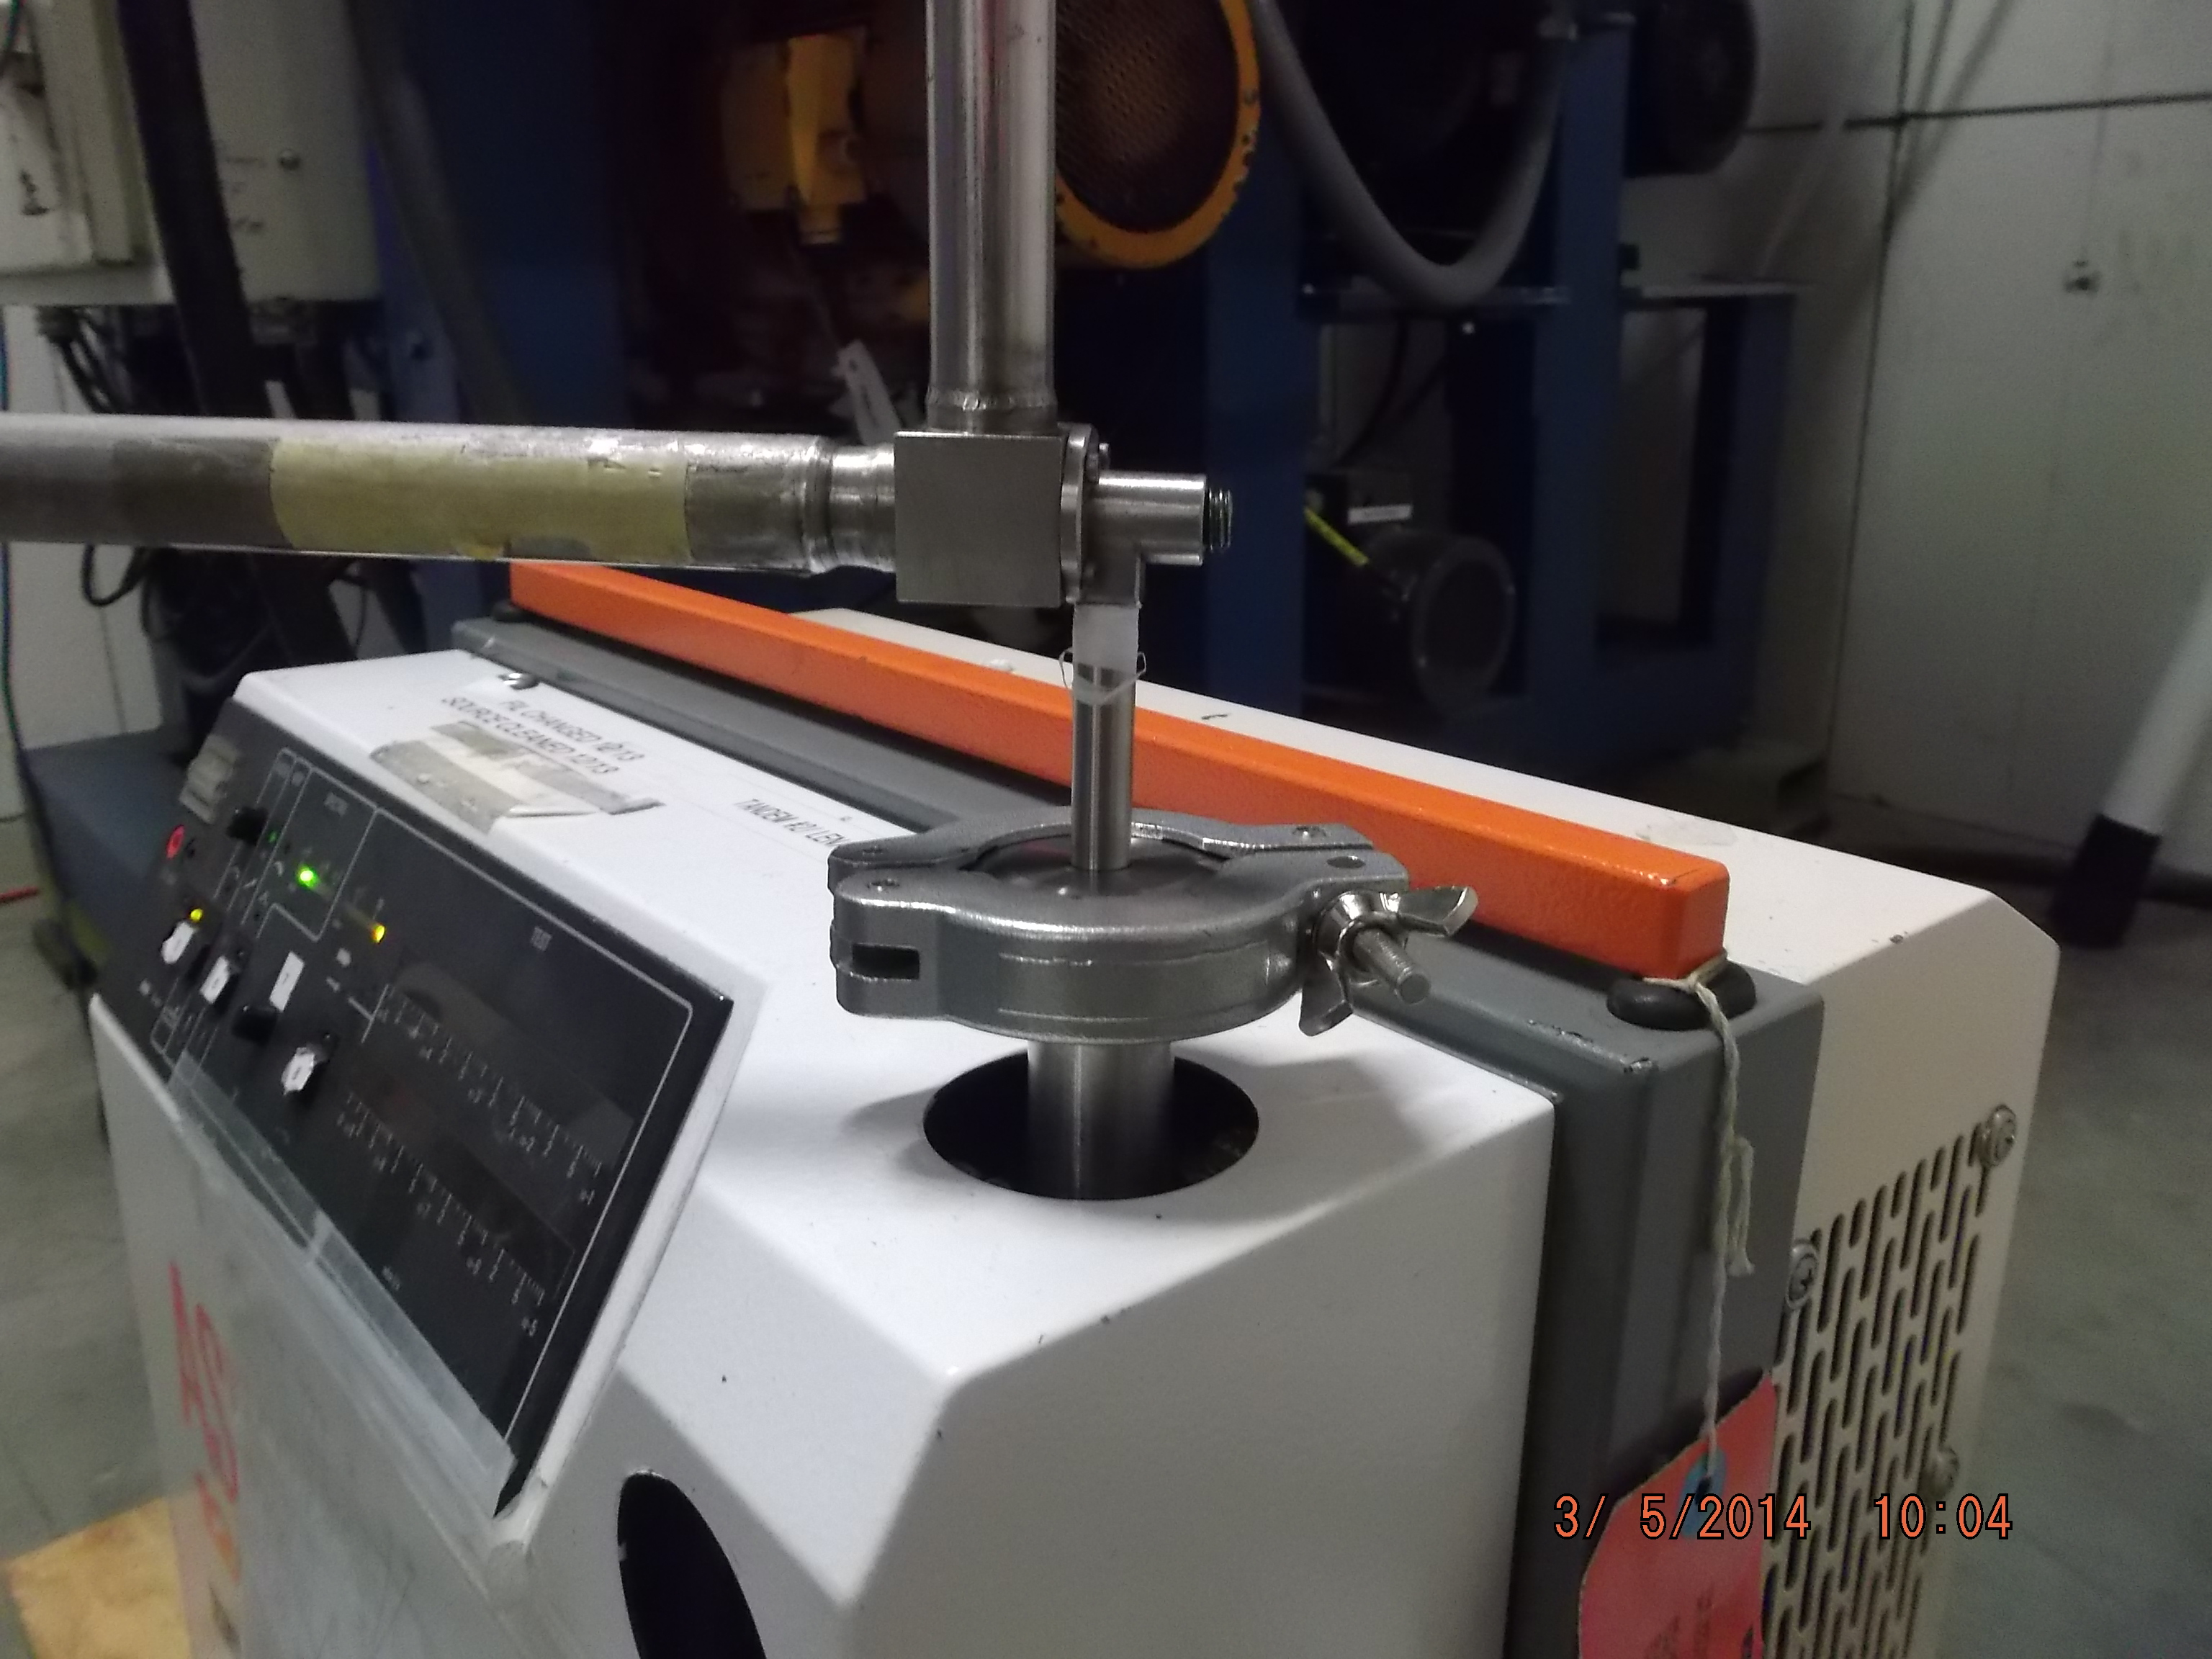
\includegraphics[width=.8\linewidth]{img/ltl-pumping.jpg}
 % ltl-pumping.jpg: 3072x2304 pixel, 72dpi, 108.37x81.28 cm, bb=0 0 3072 2304
 \caption{Pumping down the LTL.  The side screw valve is opened to allow the LD to pump the vacuum jacket.}
 \label{fig:ltl-pumping}
\end{figure}



\section{Indium Extrusion}
Hifrost requires indium wire precisely 1 mm in diameter for making MC and IVC seals.  Indium seals must be scraped away after use, and the metal is always recovered (due to its scarcity).  The Indium Association of America charges roughly \$1000 for 13 feet, or about \$20-30 per attempted seal, so it is worth creating our own wire from the so-called ``scraps''.

Indium extrusion is the name of the process that transforms bulk indium into nicely shaped wire.

\subsection{Background} 

Indium scraps or ingots are put into a hollow cylinder with a small hole in the bottom, and the indium is softened with heat and pushed through to make a 1 mm wire.  The melting point of indium is about $150 ^\circ$ C, but approaching this temperature leaves the indium ``runny'' and impossible to shape.  We have found heating the cylinder to $100 ^\circ$ C with a heating tape yields the ideal consistency.

Our first indium die, the plate at the bottom of the hollow cylinder that has a small hole for shaping indium, had a 1 mm hole.  For whatever reason, this produced indium 0.75 mm in diameter (too small for the HiFrost flanges).  We increased the die to 41 mils (about 5\% larger), and the indium wire came out at 1 mm.  

When extruding the indium, a varying force on the hydraulic pump sometimes leads to uneven wire (something like sausage links).  To prevent this, a continuous, non-varying force should be applied for an entire press.

\subsection{Materials}
The \textbf{extrusion cylinder} is an aluminum cylinder with six 1/4-20 bolt holes tapped in the bottom.  The inside of the aluminum is lined with another hollow cylinder made of steel, which precisely matches a \textbf{steel rod} that slides in and out.  If the rod and inner cylinder do not precisely fit, either the rod will not fit in the cylinder or the indium will leak out during the press.  There is a small hole drilled in the side of the aluminum for a thermocouple.

Screwed into the bottom of the extrusion cylinder is the \textbf{indium die}, a plate with a hole through the middle to push indium through.  The entrance hole in top of the die matches in the extrusion cylinder, and the exit hole in the bottom of the die shapes the indium wire.  The die is a separate component from the extrusion cylinder for cleaning and modularity reasons.

\textbf{Indium} is generally recovered from scraps of old seals or ingots are bought from the Indium Association of America (currently a pound costs \$300).  Ingots should be cut with a knife into smaller blocks to fit inside the extrusion cylinder.

The \textbf{extrusion stand} is a mounted, horizontal bar for the hydraulic press to push against so pressure is applied to the extrusion cylinder.  There must also be a hole in the base of the stand for the pressed indium wire to be collected.

A \textbf{thermocouple} sensor is used with an accompanying \textbf{thermocouple readout} to measure the temperature of the extrusion cylinder.

\textbf{Heat tapes} warm the indium so it may be pressed.  The tapes should be long enough to wrap around the cylinder to warm it evenly.

A layer of \textbf{aluminum foil} is wrapped around the heating tapes to keep the heat from dissipating away.

\textbf{Latex and clothe gloves} are for personnel safety and keeping the indium sanitary.

A \textbf{variable alternating current} unit adjusts the temperature of the heating tape.

The indium is extuded onto sterile \textbf{\com{Absorbond Wiper Sheets, TX}} 9\inches x 9\inches, 409, and kept for storage.

An \com{Enerpc} P39 Porta Power \textbf{hydraulic hand pump} provides the force for extrusion.

\subsection{Extrusion process}

\begin{figure}
 \centering
 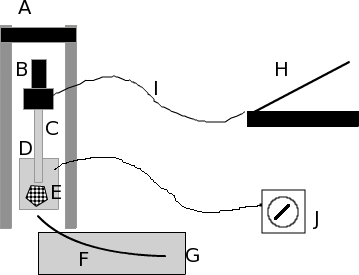
\includegraphics[scale=0.5]{img/extruder-setup.png}
 % extruder-setup.png: 359x275 pixel, 72dpi, 12.66x9.70 cm, bb=0 0 359 275
 \caption{Indium extruder setup: A) extruder stand, B) hydraulic pump, C) steel rod, D) extrusion cylinder, E) indium scrap/ingot fragments, F) finished wire exiting die, G) sterile wipe sheet, H) hand jack, I) hydraulic line, J) thermocouple gauge}
 \label{fig:extruder}
\end{figure}

\begin{figure}
 \centering

\begin{minipage}[b]{0.45\linewidth}
 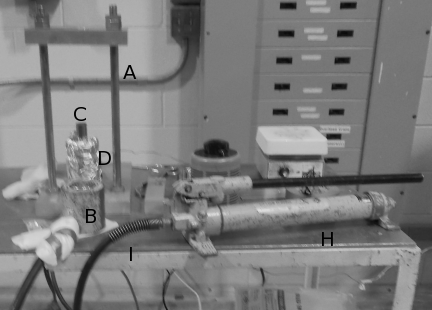
\includegraphics[width=\linewidth]{img/extruder-setup-photo.png}
 \caption{A photo of the setup.}
 \label{fig:extruder-setup-photo}
\end{minipage}
\quad
\begin{minipage}[b]{0.45\linewidth}
 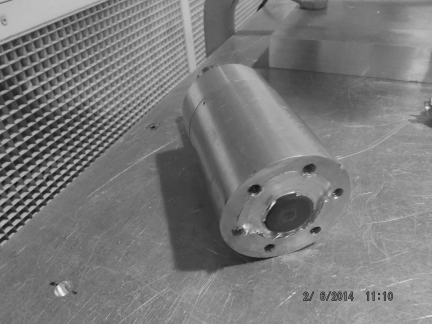
\includegraphics[width=\linewidth]{img/extruder-cylinder.png}
 % extruder-setup.png: 359x275 pixel, 72dpi, 12.66x9.70 cm, bb=0 0 359 275
 \caption{The extruder cylinder without the die.  The steel rod is plunged all the way down and leftover indium can be seen on the surface.}
 \label{fig:extruder-cylinder}
\end{minipage}
\end{figure}


\begin{enumerate}
\item Prepare electrical connections for heating tape and thermocouple gauge and readout.
\item Remove steel rod from extrusion cylinder and insert blocks of indium.  Place the steel rod back in the cylinder.  \textit{NB: after losses, 100 grams of indium provides approximately 10 feet of wire instead of the theoretical 50 feet.}
\item Wrap the cylinder with heating tape and aluminum foil.
\item Place the cylinder/rod under the extrusion stand.
\item Set the variable current source so the heating tape reaches about $70^\circ$ C, which takes around 20 minutes.  Increase the temperature in steps, allowing the thermocouple to equilibrate between steps, to $100 ^\circ$ C.  \textit{NB: on our VariAC unit the 50 mark corresponds to $75 ^\circ$ C and the 60 mark corresponds to $100^\circ$ C}
\item Set the hydraulic jack on the extrusion cylinder and under the stand's horizontal bar.
\item Use the hand jack to slowly push the indium through the extrusion cylinder and out the die.  The press takes about 5 minutes.  A second person slowly winds the indium wire on the wiper sheets. 
\end{enumerate}


\begin{figure}
 \centering
 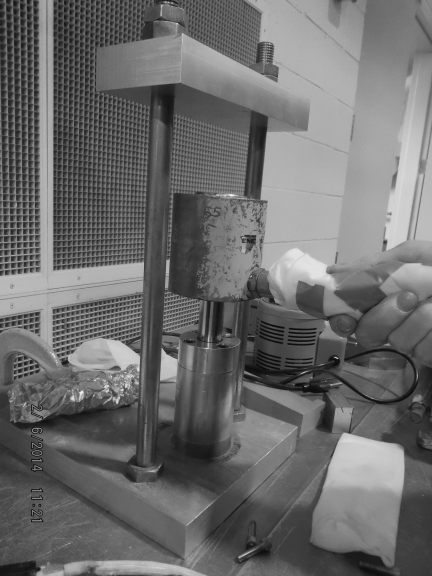
\includegraphics[scale=0.75]{img/extruder-demo.png}
 % extruder-setup.png: 359x275 pixel, 72dpi, 12.66x9.70 cm, bb=0 0 359 275
 \caption{The hydraulic press sitting on top of the extrusion cylinder.}
 \label{fig:extruder-demo}
\end{figure}


\section{Making Indium Seals}


\begin{enumerate}
 \item First, clean both flanges the indium will seal together.
 \item Measure the diameter of the indium to be used; it should be 1 mm
 \item Cut a length just greater than the circumference of the flange (MC: 158 mm; IVC: 271 mm) plus a centimeter or two.  Do not allow the indium wire to touch any dirty surfaces.
 \item Wrap the wire around the proper aluminum setting tool.
 \item Using a razor blade, cut the wire at an angle as in Figure \ref{fig:indium-cut}, firmly placed on the aluminum block.
 \item Flip the mating can (IVC or MC bell housing) upside down and press firmly to the aluminum block TODO photo.
 \item Turn the parts so the aluminum block is on top, and carefully remove the block so the indium is transferred to the can.  Check to make sure the wire was not shifted, especially where the two ends meets.
 \item When it is time to make the seal on the fridge, carefully raise the can up to the fridge within 1 cm from touching, not allowing anything to touch the indium wire.  If the wire is displaced, begin from the beginning.  Hold in place with a chemistry clamp. TOOD show photo
 \item Insert two appropriate machine screws up through the can, and turn twice so they can support the weight of the can without the chemistry clamp.  The indium should not touch the fridge flange.
 \item Remove the clamp and turn the remaining four screws 2 times each.
 \item Alternate tightening the screws 1/4 turn each in a ``star'' pattern.  That is, do not turn adjacent screws consecutively, and no single screw is tightened twice unless the other five screws have been tightened in between.
 \item When the indium is compressed, make sure all the screws are evenly tightened, but do not strip the machine screws' hex heads.
 \item If possible, leak check the indium seal.
\end{enumerate}

\begin{figure}
 \centering
 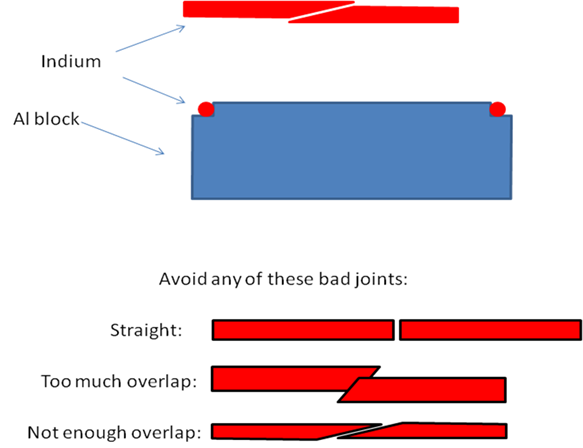
\includegraphics[scale=0.5]{./img/indium-cut.png}
 % indium-cut.png: 583x448 pixel, 96dpi, 15.42x11.85 cm, bb=0 0 437 336
 \caption{How to cut indium wire for fridge seals. \cite{zhaoindium}}
 \label{fig:indium-cut}
\end{figure}



\section{Breaking Indium Seals}
\begin{enumerate}
 \item Remove screws with 1.5 mm allen key and the modified MC wrench.  Visually inspect each screw for indium or signs of stripping, and turn each nut back on the screw it came off of.  If there is any torque resistance or sign of stripping, the screw was likely damaged when the indium seal was tightened and both the screw and nut should be discarded.  If there is no damage, return the nuts/screws to the bag labeled ``MC Screws and Nuts''.
\item Use two MC screws and the 1.5 mm allen key as jacking screws the break the indium seal.  Defining the top of the fridge (in the horizontal orientation) as 12:00, the jacking screw holes are at 1:00 and 5:00 look upstream.  The jacking screw holes can be identified by threaded holes in the MC bell housing that have no matching through holes on the fridge MC flange.  Alternate between screws making 1/4 turns until the MC is free.
\item Remove the MC from the fridge, careful not to damage the sensors on the copper dam.
\item Remove the jacking screws from the MC and place in the bag labeled ``MC Screws and Nuts''.
\item Scrape indium, if any, off the MC and place the MC in the safety zone.
\item Scrape indium off the fridge flange, recovering as much as possible in the indium scrap container; be very careful not to touch the stainless steel beam window.
\end{enumerate}


\section{Magnet Lead Installation}

\section{Mounting Fridge}

\section{Dismounting Fridge}

\section{Cleaning Viton/Buna O-rings and Grooves}

HiFrost only uses isopropyl alcohol for cleaning vacuum parts.  Methanol bottles are scattered around DFELL, but they are not to be used.

Most o-ring encountered are for KF joints.  It is not practical to clean every o-ring every time it is touched, and this is unnecessary because our vacuum system is not UHV, so most KF joints can be visually inspected for dirt before use.


\vsepfbox{\parbox{.93\textwidth}{\centering
\textbf{All \het{} system o-rings must be leak checked every time they are taken apart, regardless of whether they were cleaned or not.}
}}

To clean a KF o-ring:
\begin{enumerate}
 \item remove o-ring from center piece
 \item moisten a Kim Wipe with isopropyl alcohol
 \item gently pinch the o-ring with the wipe, rotating it around to clean the whole surface
 \item replace the oring over the centerpiece
 \item wipe down the outside of the o-ring one more time
 \item reassemble the KF joint, trying to touch only the centerpiece as much as possible (tip: gravity is your friend, here)
\end{enumerate}


\subsection{Fridge flanges}
The triple flange, \het{} back flange, evaporator pumpout and \het{} pumpout all have rubber o-rings set in grooves.  If any of these leak the fridge will not be able to acheive dilution (or \het{} will leak out), but they cannot be leak tested during a cold-target run because there is no time to pump down the system with a leak detector.

To minimize the change of them leaking, the following should be done each time one of these flanges are opened:

\begin{enumerate}
 \item clean o-ring with isopropyl alcohol as described above
 \item dampen qtip with alcohol and swap out o-ring groove (this will be very dirty from vacuum grease)
 \item use a minimal amount of vacuum grease to coat the o-ring all the way around
 \item replace the o-ring and seal the flange immediately
\end{enumerate}

The vacuum grease feels unpleasant on hands, so latex gloves may be used.  Otherwise, be sure to wash up afterward so vacuum grease doesn't contaminate other fridge components.



\section{Changing Kenol Connectors}

\section{Installing Heating Tapes}

\section{Filling \lnn{} Trap}

\section{Check 250LD/500LD LHe Level}
\label{procedure:check-lhe-level}
The LHe level of helium dewars is checked upon delivery and after they are used to fill the 500LD. The 500LD LHe level is checked after it is filled, after initially filling the 100LD and periodically throughout the run. The 100LD has an internal level probe installed and does not use this procedure.

\begin{enumerate}
 \item Remove zip ties and plastic wrap on full 250LD.
 \item Make sure there is nothing sensitive directly above the dewar, then release pressure by opening main flow valve on top of the dewar. A large, cold plume will exhaust pressurized helium gas.
 \item Use cryogenic gloves to slowly lower the level probe into the main flow valve. A smaller cold plume will exhaust upwards as the level probe cools down.
 \item Plug the level probe into the level probe readout and record the reading. As a sanity check, lift the level probe a few inches to make sure the readout changes correspondingly.
 \item Disconnect the level probe and remove it from the 250LD, storing it where it can safely warm up.
 \item Close the main flow port.
\end{enumerate}

\section{Attach Pressurization Line to LHe Dewars}
\label{procedure:attach-pressurization-line}

The 250LD and 500LD have LHe pushed out of them by pressurizing the top of their liquid contents with helium gas.  The helium gas pushes down on the liquid surface, pushing liquid up a transfer line and out of the dewar.

The procedure below ensures air will not get in to the pressurization line and freeze the dewar port.

\begin{enumerate}
 \item Check that the pressurization cylinder is not empty and a full helium cylinder is nearby.  Make sure the regulator has single PSI increments discernable.
 \item Open the pressurization cylinder and set the regulator to 2 PSI.  Verify helium gas is flowing out.
 \item Slowly open the dewar pressurization valve on the to-be-pressurized dewar until pressurized gas begins to flow out at about 5 PSI.  If the pressurization frosts, close it and wait until it warms up, using a heat gun only if  necessary.
 \item With gas coming out of both the dewar pressurization port and the pressurization cylinder, mate the two connectors and close the dewar pressurization valve.
\end{enumerate}


\section{Purging Helium Lines}

\section{Vacuum Rise Testing}

A leak checker is the proper way to determine if a vacuum volume is leak tight.  However, it is not always practical and sometimes very difficult to leak check a large volume, so we use a vacuum rise test as a course characterization of the vacuum fidelity.


The concept is to pull a vacuum down in a volume, isolate it from the pump, then watch if the vacuum rises.  Outgassing and a leak are generally the only two effects we will see, but outgassing usually stops the pressure rise far below 1 atm.

To set up, gather the following:
\begin{itemize}
 \item pump 
 \item associated KF vacuum fittings/hoses
 \item KF pressure gauge
\end{itemize}


\begin{figure}[h]
 \centering
 \begin{minipage}{.45\textwidth}
 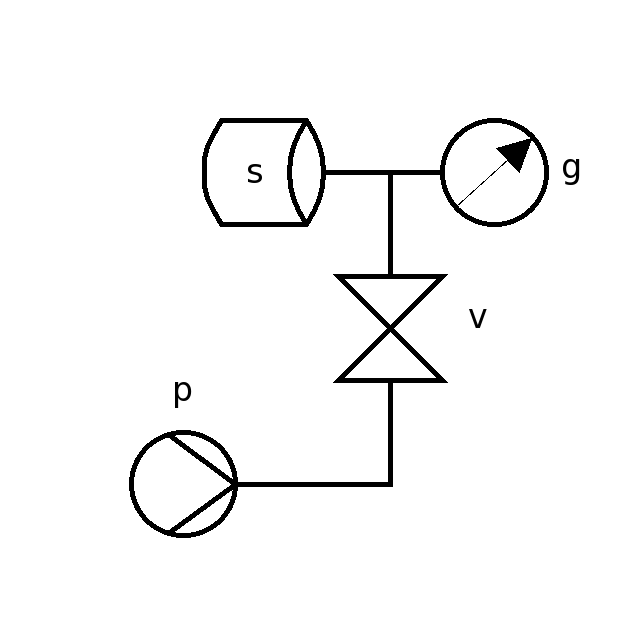
\includegraphics[width=\textwidth]{./img/vacuum-rise-system.png}
 \caption{Vacuum rise schematic: \textit{s} is the system to check; \textit{g} is a pressure gauge; \textit{}v is a leak-tight manual valve; \textit{p} pumps to atmosphere.}
 \label{fig:vacuum-rise-system}
 \end{minipage}
 \quad
 \begin{minipage}{.45\textwidth}
 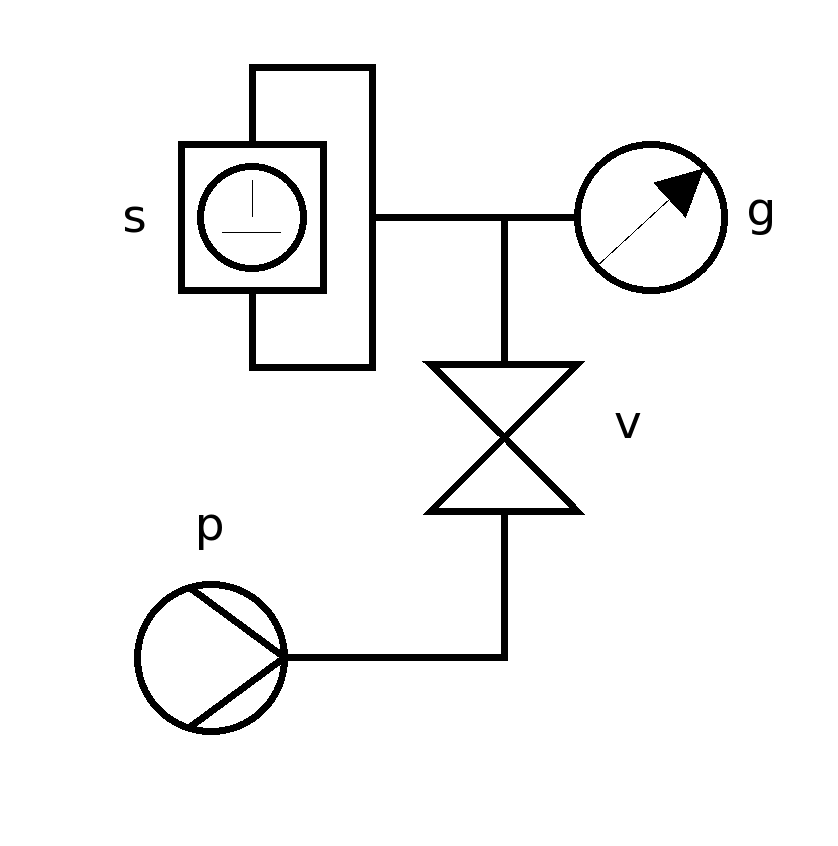
\includegraphics[width=\textwidth]{./img/vacuum-rise-dual-system.png}
 \caption{The same as Figure \ref{fig:vacuum-rise-system} except \textit{s} has two ports, the inlet and exhaust of a pump, in this case.}
 \label{fig:vacuum-rise-dual-system}
 \end{minipage}
\end{figure}

The procedure is
\begin{enumerate}
 \item Set up as shown in Figure \ref{fig:vacuum-rise-system} or Figure \ref{fig:vacuum-rise-dual-system}.  If the system is powered (such as a pump), make sure it is unplugged.
 \item Open \textit{v} and pump down \textit{s} until the pressure gauge \textit{g} stops decreasing.
 \item Close \textit{v} and turn off \textit{p}.
 \item Monitor \textit{g} until it stops rising.  This can take from minutes to days.
\end{enumerate}

If the system \textit{s} is tight it will outgas to tens of mbar (depending on if it is contaminated with oil, water, etc) then stop.  If it is necessary (and possible), \textit{s} should then be checked with a leak detector to verify it is helium tight.

If the pressure gauge reaches an atmosphere, there is a leak in \textit{s}.  The time this takes determines how big the leak is.  A quick way to verify \textit{s} contains the leak is replacing it with a blank off and repeating the vacuum rise test.  If \textit{g} reaches an atmosphere again, there is a leak in the plumbing which should be repaired before trying the vacuum test again.

\section{Stripping Fridge}

\section{Assembling Fridge}

When putting the fridge together, there are two primary concerns: forgetting to install something (e.g., superinsulation, microwave guide support) and leaky seals.  This section does not include a cold target load and assumes the fridge is hanging vertically on the fridge stand in the Vault.

\subsection{MC}
\paragraph{Tools}
\begin{itemize}
 \item qtips/wire cutters/isopropyl alcohol
\item indium scrap box
\item 1.5 mm allen key
\item MC open faced allen wrench (4.0)
\item MC
\item 1 mm indium wire
\item chemistry clamp
\item TODO sizes for MC nuts and bolts
\end{itemize}

Read the section on making indium seals.

Hold the MC in place with the chemistry clamp so the bell housing is about 1 cm from touching the fridge flange.  Place the bolts through the MC holes and gently tighten the nuts one or two turns so the bolts don't fall.  Inspect the indium wire to make sure it is still in place, then tighten the nuts in a ``star'' pattern (never tightening adjacent screws consecutively).  Hold the bolts with an allen key while turning the wrench so the heads do not strip.  Use only the special MC wrench so the fridge does not scratch.

\begin{figure}
 \centering
 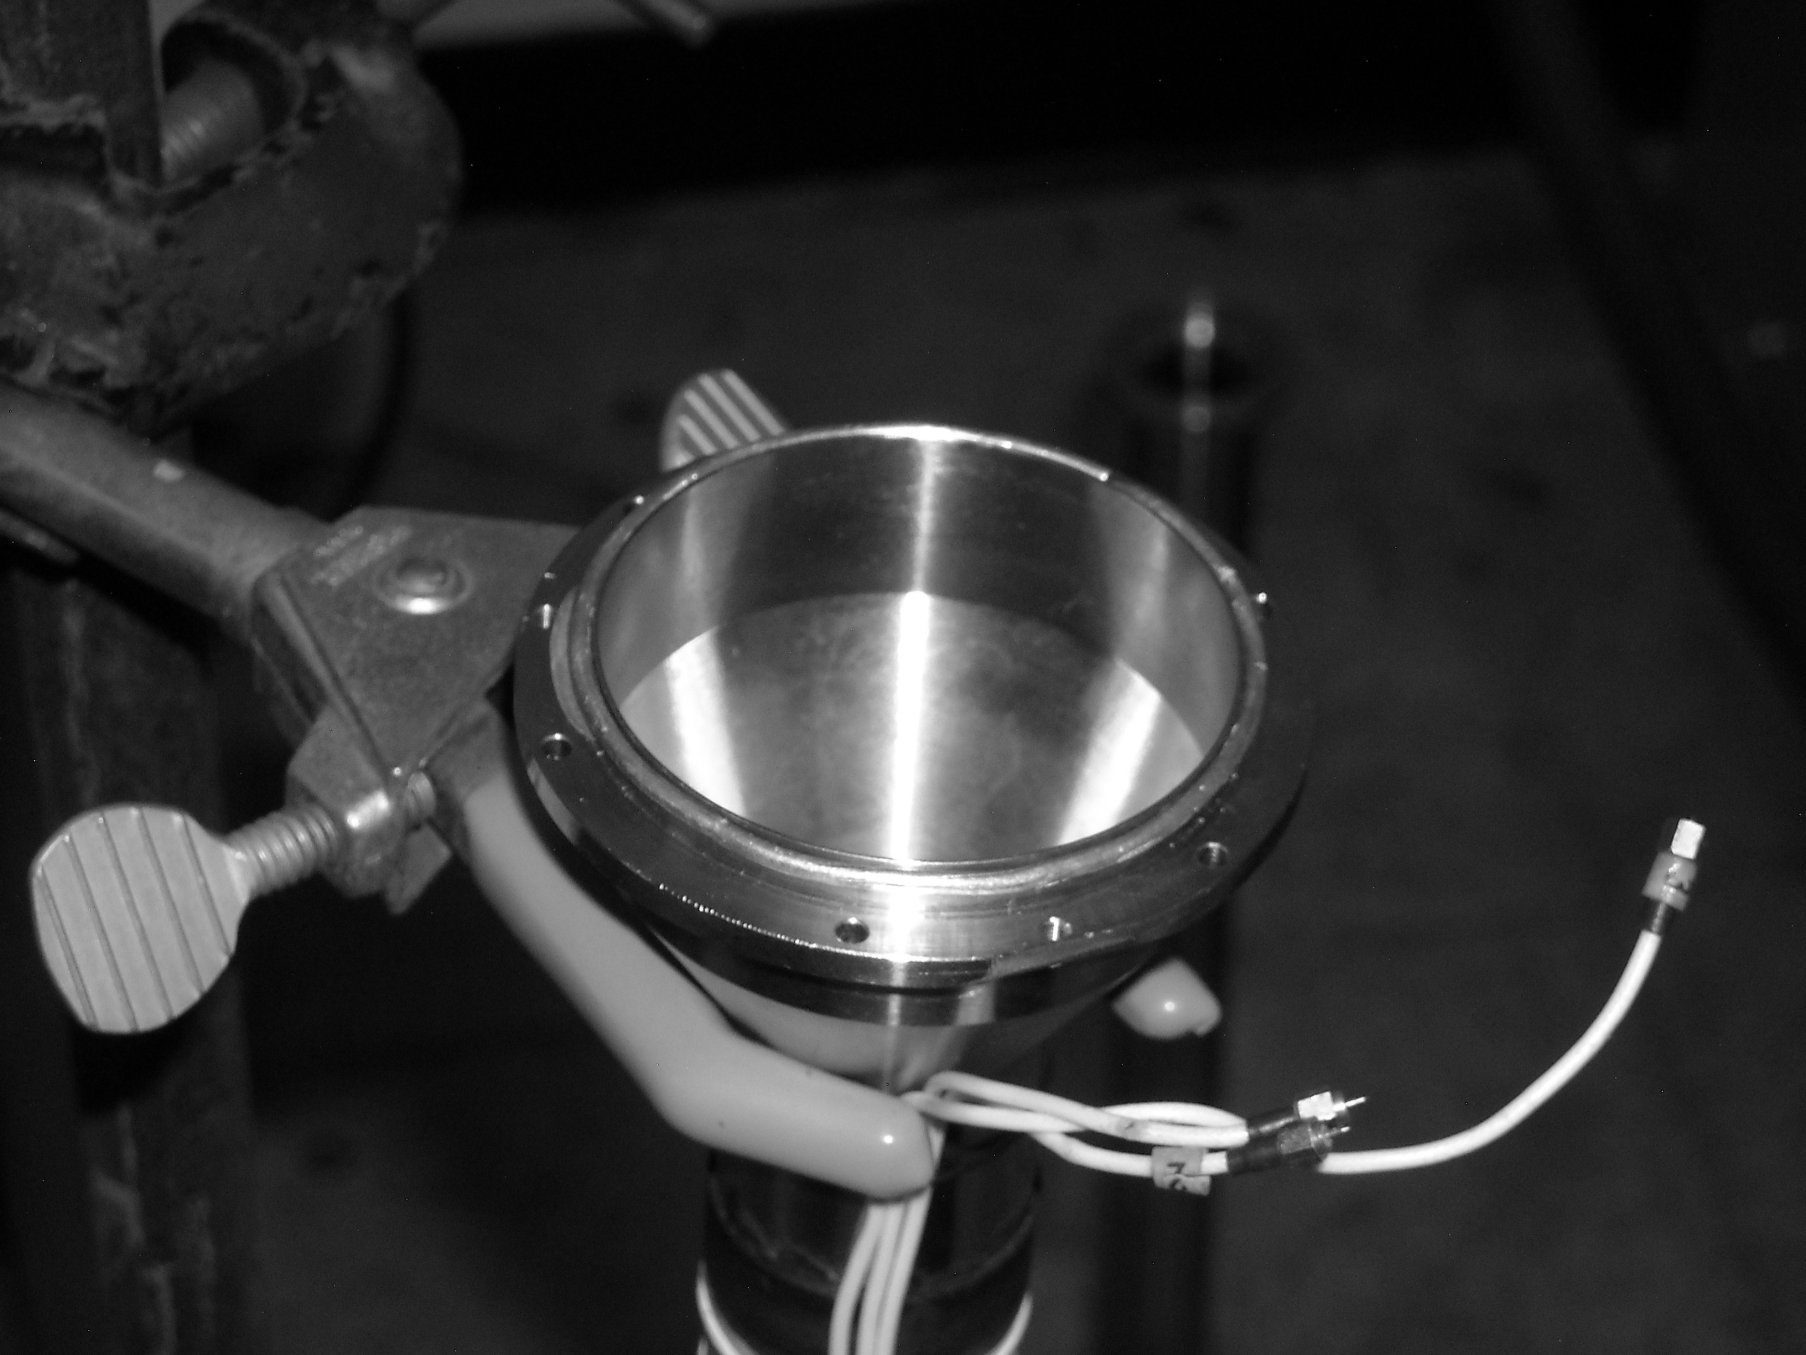
\includegraphics[scale=.75]{img/mc-stand.jpg}
 % mc-stand.jpg: 560x420 pixel, 300dpi, 4.74x3.56 cm, bb=0 0 134 101
 \caption{The MC with a prepared indium seal behind held by a chemistry clamp.}
 \label{fig:mc-stand}
\end{figure}


If loading conditions permit, leak check the MC before moving on.

  \subsection{Microwave Guide Support}
\paragraph{Tools}
\begin{itemize}
 \item small flat head screwdriver
\item squeeze-to-open tweezers
\end{itemize}

Three brass screws are usually stored in the threaded struts on the fridge where they fasten the waveguide support in place.

After unscrewing them, raise the microwave guide support over the MC making sure the waveguide is lined up with both the slot in the MC bellhousing and the circular waveguide connector on the fridge.  One person holds the support while another tightens the screws.  Hold the screws with tweezers to prevent dropping them down towards the MC (if this happens, you must start over, careful not to damage the fridge with the loose screw while taking off the support).  Warning: the microwave guide support can still fall off when it is being held by one screw.

Make sure the waveguide (or the support) is not touching the MC.  Normally this will not happen unless the support has been deformed.

  \subsection{IVC}

\paragraph{Tools}
\begin{itemize}
 \item solder station
\item 2.5 mm allen key
\item indium scrap box
\item qtips/wire cutters/isopropyl alcohol
\item TODO find out IVC screw sizes
\end{itemize}

Read the section on making indium seals.

Similar to installing the MC, first prepare the IVC indium seal and place it in the groove on the IVC flange.  One person holds the IVC within about 1 cm from the fridge while another puts in the screws.  Initially, only turn in 2 diametrically opposite screws 1 or 2 turns each so they support the IVC and it no longer needs to be held by another person.  Turn in the other 4 screws 1 or 2 turns each.  Inspect the indium seal to make sure it is still in place (it should not be touching the fridge flange yet) before turning in the screws in a ``star pattern'' similar to the MC.  Be careful not to strip the screw heads.


Leak check if possible.


\subsection{OVC}

\paragraph{Tools}
\begin{itemize}
 \item pliers for pilot pins
\item 5 mm allen key
\item three OVC cans (inner, outer, nose cone)
\item triple flange orings
\item pilot pins
\item 2x nut plates
\item triple flange screws TODO find size
\end{itemize}

Make sure the orings and grooves are clean (see cleaning orings section).  Place the outer OVC can on the blue fridge lift in the Vault, and lower the inner OVC can inside of it, making sure the black lines on the flanges line up.  Place the pilot pins up through the pilot holes and secure the cans in place with nuts and threaded rod that fit through the fridge lift platform.  Hook up the OVC manifold to the pumpout (making sure the hose is coming off at the appropriate angle for Blowfish clearance) and warm up the OVC turbo pump.  Raise the nose cone in place, being sure to line up the large dents, and begin pumping.  Leak check the OVC.


With the OVC still being pumped, remove it from the fridge lift and raise it over the fridge.  Line up the black lines on the triple flange and push the pilot pins in by hand, using pliers if they need to be rotated or pulled out slightly.


Loosely turn in all the triple flange screws, careful not to strip the aluminum taps.  Tighten in a star formation so the oring does not become unevenly compressed.

\section{Removing/Replacing \het{} Baffles}